\documentclass[10pt]{article}

\usepackage[utf8]{inputenc}

\usepackage{textcomp}
\usepackage[T1]{fontenc}
\usepackage{multirow}
\usepackage{float}
\usepackage[caption = false]{subfig}
\usepackage{longtable}
\usepackage{listings}
\usepackage{mathtools}
\DeclareMathOperator{\tr}{Tr}
\usepackage{commath}
\usepackage{bbold}
\usepackage{xcolor}
\usepackage{physics}
%\usepackage[margin=1.8cm]{geometry}

\usepackage{tikz-cd}
\usepackage{amsmath}
\usepackage{amsfonts}
\usepackage{amssymb}
\usepackage{amsthm}
\usepackage{graphicx}
\usepackage[colorinlistoftodos]{todonotes}
\usepackage[colorlinks=true, allcolors=blue]{hyperref}
\usepackage{siunitx}
\sisetup{separate-uncertainty=true}

\usepackage[sc]{mathpazo}
\linespread{1.05}         % Palladio needs more leading (space between lines)
\usepackage[T1]{fontenc}

\newcommand{\diag}[1]{\text{diag}\qty(#1)}
\newcommand{\const}{\text{const}}
\newcommand{\sign}[1]{\text{sign}\qty(#1)}
\renewcommand{\H}{\mathcal{H}}
\renewcommand{\dim}{\text{dim}}
\newcommand{\C}{\mathbb{C}}
\newcommand{\R}{\mathbb{R}}
\newcommand{\N}{\mathbb{N}}
\newcommand{\Z}{\mathbb{Z}}

\renewcommand{\var}[1]{\text{var} \qty(#1)}
\newcommand{\average}[1]{\langle #1 \rangle}

\newcommand\mybox[1]{%
  \fbox{\begin{minipage}{0.9\textwidth}#1\end{minipage}}}


\begin{document}

%\section*{Resonances}

Jacopo Tissino, 1152348, 22 June 2019. The images used come from the slide presentation by Donatella Lucchesi.

\textbf{Describe the concept of \emph{resonance} in particle physics, the Breit-Wigner distribution and its use in data analysis.}

Many particles we would like to study are not stable, but are instead in shallow
minima of their potential: they can tunnel or be excited easily through the potential barriers, and decay before they can be observed moving through space.

We can study them in the brief period of time between when they are formed and when
they decay: suppose we have a process \(\ce{a} + \ce{b} \rightarrow O \rightarrow \ce{c} + \ce{d} \), where \(O\) is the metastable state we want to study.

We expect the cross section to be higher if a metastable resonant state is formed: the probability of going from \(\ce{a}  + \ce{b}  \) to \(\ce{c} + \ce{d} \) directly will be less than the probability of the process happening through \(O\).

This qualitative statement can be formalized:

\begin{equation} \label{eq:breit-wigner}
    \sigma(E)  =
    \frac{(2J+1)}{(2s_a + 1) (2s_b + 1)} \frac{4 \pi }{E^2}
    \frac{\Gamma_i \Gamma_f}{(E-M_R)^2 + (\Gamma/2)^2}
\end{equation}

where

\begin{itemize}
    \item \(\sigma\) is the scattering integral cross section, which is calculated as \((\#\text{events} - \#\text{background events})/ L\), where \(L\) is the time-integrated luminosity;
    \item \(E = \sqrt{s} \) is the center of mass energy;
    \item \(J\) is the spin quantum number of the resonant state;
    \item \(s_{a, b}\) are the spin quantum numbers of the reacting particles: these spin terms are included to account in order to average over all possible polarizations of the incoming particles;
    \item \(\Gamma_{i,f}\) are the initial and final partial widths of the reaction, respectively the width for \(\ce{a} + \ce{b} \rightarrow O\) and \(O \rightarrow \ce{c} + \ce{b} \),
    \item \(\Gamma\) is the resonance width: the square modulus of the wavefunction of the resonance contains the term \(\exp(- \Gamma t) \),
    \item \(M_R\) is the mass of the resonant state.
\end{itemize}

Note that the Breit-Wigner formula comes from a first-order expansion, so it is only valid near the peak: when \(\abs{E-M_R} \gg \Gamma \) we cannot use it.

An example of application of this formula was the discovery of the \(\Delta\) baryon: when colliding \(\pi^{\pm}\) on a fixed proton target, we see a resonance at an energy of \SI{1236}{MeV}: if we plot the scattering cross section \(\sigma\) against the center of mass energy \(E = \sqrt{s} \) we see a peak, which corresponds to \(E = M_R\).

\begin{figure}[H]
    \centering
    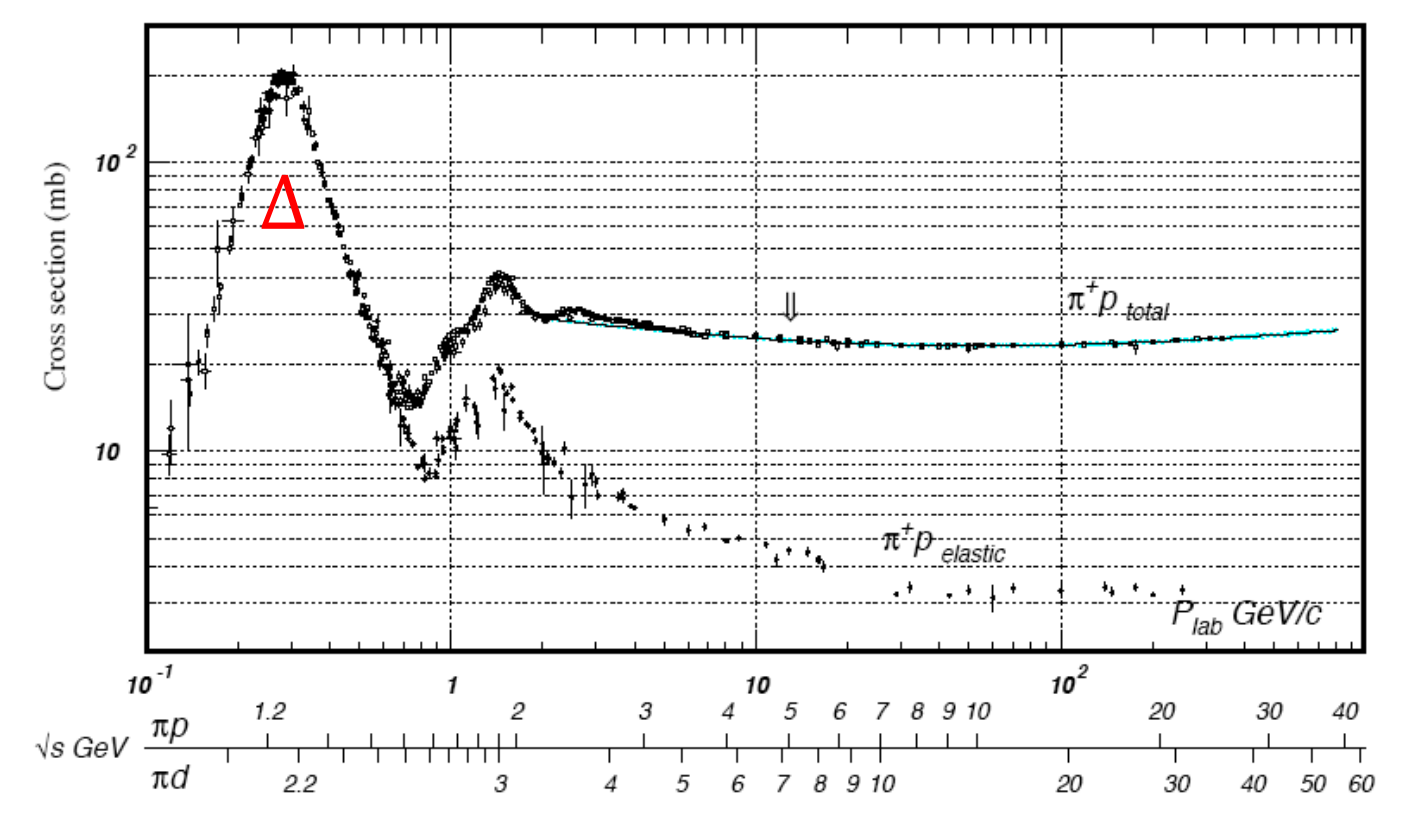
\includegraphics[width=0.5\textwidth]{breit-wigner.png}
    \caption{Resonance peak corresponding to the \(\Delta\) baryon.}
    \label{fig:delta-baryon}
\end{figure}

Another way to find resonances in reactions of the form \(\ce{a} + \ce{b} \rightarrow \ce{R} + \ce{e} \rightarrow \ce{c} + \ce{d} + \ce{e} \), that is, some of the times the reaction occurs it passes through the metastable state \(\ce{R} \) which decays into \(\ce{c} + \ce{d}\).

This reaction path will be favoured over others, so we can histogram the number of events we see at each value of the invariant mass of the particle pair \(\ce{c} + \ce{d}\).

\begin{figure}
    \center
    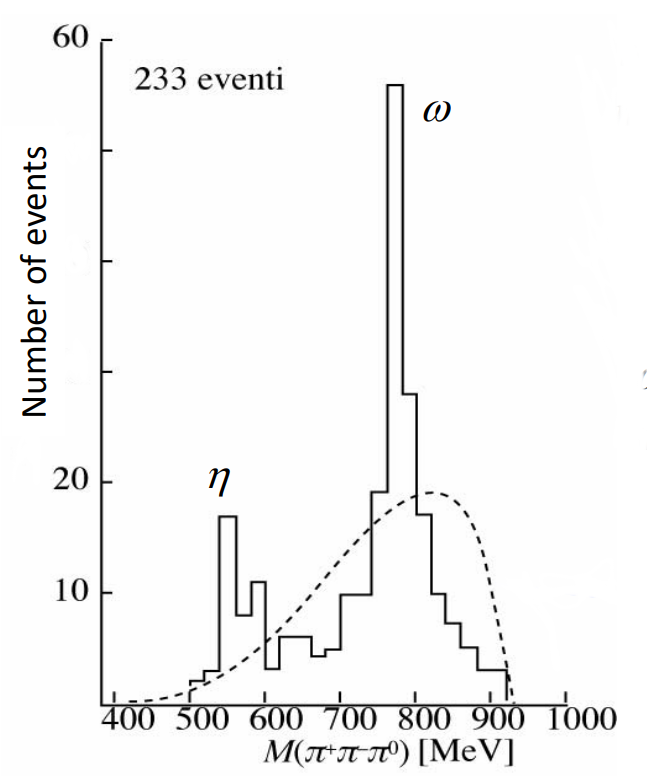
\includegraphics[width=0.34\textwidth]{eta.png}
    \caption{Resonances in Bevatron bubble chamber. Number of events is plotted against the invariant mass of the \((\pi^+ + \pi^+ + \pi^0)\) system. The dotted line represents the phase-space volume corresponding to the invariant mass, normalized in order for it to have integral \(N=233\).}
    \label{fig:bevatron}
\end{figure}

This was used, for example, in the study of a beam of \(\SI{1.23}{GeV/c} \) \(\pi^+\) going into a bubble chamber of liquid deuterium. The reaction is

\begin{equation} \label{eq:process}
    \pi ^+ + \ce{d} \rightarrow
    x + \ce{p}  + \ce{p}
    \rightarrow \pi^+ + \pi^- + \pi^0 + \ce{p} + \ce{p}
\end{equation}

and we assume the new particle \(x\) decays into \(\pi^+ + \pi^- + \pi^0 \) so we look at the histogram with respect to the invariant mass of this combination.
We would expect to get the curve of the Lorentz-invariant phase-space volume corresponding to the differential mass \(\dd{m} \):

\begin{equation}
    f(m) \propto
    %\frac{1}{(2 \pi)^9}
    \int \frac{\dd[3]{p_{\pi^+}}\dd[3]{p_{\pi^-}}\dd[3]{p_{\pi^0}}}
    {8E_{\pi^+}E_{\pi^-}E_{\pi^0}}
\end{equation}

where the integral extends over all of the combinations of phase-space coordinates such that
\(m \leq \sqrt{(\sum E_i)^2 - (\sum p_i)^2} \leq m + \dd{m}\) (\(i\) labels the three \(\pi\) particles).

This will have some smooth shape, and we can calculate its bounds knowing the momentum of the \(\pi^+\) is \(\SI{1230}{MeV}\), the masses of the \(\pi^{\pm}\) are \SI{139.570}{MeV}, the mass of the \(\pi^0\) is \SI{134.977}{MeV}, the mass of the deuton is \SI{1875.612}{MeV}, the mass of the proton is \SI{938.783}{MeV}.

Then, then energy of the incoming beam will be \(E_{\pi^+} = \SI{1238}{MeV}\) and we will have \(\sqrt{s} = \sqrt{
(E_{\pi^+} + m_d)^2 - p_{\pi^+}^2
} \approx \SI{2860}{MeV} \).

Surely the invariant mass \(m = m(\pi^+ + \pi^- + \pi^0)\) will not be less than the sum of the \(\pi\) masses, which equals \(m(\pi^+) + m(\pi^-) + m(\pi^0)=\SI{414.12}{MeV} \leq m\).

Also, we must have \(m + m_d \leq \sqrt{s} \). This means \(m \leq \SI{984.6}{MeV} \).

Instead of a smooth curve between these extremes, we see two definite peaks: the results are shown in figure \ref{fig:bevatron}.

We fit each peak with a Lorentzian, whose FWHM is \(\Gamma\), and whose center is \(E_R\). These correspond to two possible \(x\) particles in the process \eqref{eq:process}: the fit results are shown in table \ref{fig:decay-pi}, labelled by the names of the two particles.

\begin{table}[H]
    \centering
    \begin{tabular}{c|c|c}
            & \(E_R\) &  \(\Gamma\) \\
            \hline
        \(\omega\) &  \SI{782}{MeV}  &   \SI{8}{MeV}    \\
        \hline
        \(\eta\) &  \SI{548}{MeV}    &   \SI{1.3}{MeV}    \\
    \end{tabular}
    \caption{Fit parameters for the particles which decay into \(\pi^+ + \pi^- + \pi^0 \).}
    \label{fig:decay-pi}
\end{table}

Thus, through a Breit-Wigner fit we can very precisely measure the properties (mass and average lifespan) of a resonant state which only exists for an incredibly short time: for example, the \(\eta\) has \(\Gamma=\SI{1.3}{MeV} \), so its lifespan is of the order \(\tau = \hbar/\Gamma \approx \SI{5e-22}{s}\).

%
% We derive the formula \eqref{eq:breit-wigner} in the case \(\ce{a}, \ce{b} = \ce{c}, \ce{d}\).
% Recall the fact that, if the incoming wavefunction is a planar wave and the outgoing function is of the form \(\psi =  f(\theta, \varphi) \exp(pr/i \hbar) / r \), then the differential scattering cross section is
%
% \begin{equation}
%     \dv{\sigma}{\Omega} = \abs{f(\theta, \varphi)}^2
% \end{equation}
%
% In our case the widths are all the same, \(\Gamma = \Gamma_i = \Gamma_f\), since there is only one transition type. It can be shown %by Fourier transforming the potential?
% that to first order
%
% \begin{equation}
%     f = \frac{E_R - E}{\Gamma/2}
% \end{equation}
%
% The factor \(4 \pi (2J+1) / k^2\) comes from an optical analysis.
%
% The factor \(1/(2s_a+1) (2s_b+1)\) comes from summing over the spin states.

\end{document}
